\chapter{Theoretische Grundlagen f�r die Modellierung}

In diesem Kapitel sollen die in der Arbeit verwendeten mathematischen Hilfsmittel vorgestellt werden und die wichtigsten Eigenschaften bewiesen werden. Dabei werden Grundlegende Kenntnisse im Bereich der Wahrscheinlichkeitstheorie vorausgesetzt und dass Begriffe wie Wahrscheinlichkeitsraum, Zufallsvariable, Dichte- und Verteilungsfunktion bekannt sind. Im Folgenden sei stets der Wahrscheinlichkeitsraum $(\Omega,\mathfrak{A},\mathbb{P})$ gegeben. Wir bezeichnen f�r eine Zufallsvariable $X: \Omega \rightarrow \mathbb{R}$, die Abbildung $F_X:\mathbb{R} \rightarrow [0,1]$, welche definiert wird durch
\begin{eqnarray*}
		F_X(x):=\mathbb{P}(X\leq x),
\end{eqnarray*}
als \textbf{Verteilungsfunktion} von $X$. Wir schreiben $X \sim F_X$, wenn $F_X$ die Verteilungsfunktion von $X$ ist. Des Weiteren ist 
\begin{eqnarray*}
		\overline{F}_X(x):=1-F_X(x) = \mathbb{P}(X > x)
\end{eqnarray*}
die Schwanzfunktion von X.
\\

\section{Verwendete Verteilungen}
Zun�chst werden wir die Verteilungen vorstellen, die in dieser Arbeit verwendet werden, und die wichtigsten Eigenschaften vorstellen.
\\

\begin{defini}
Eine Zufallsvariable $X:\Omega\to \mathbb{R}$ hei�t \textbf{exponentialverteilt zum Parameter $\lambda$} (kurz: $X \sim exp(\lambda)$), wenn sie die folgende Dichtefunktion besitzt:
	\begin{eqnarray*}
		f_\lambda(x)=
		\begin{cases}
			\lambda e^{-\lambda x} & \text{f�r } x\geq 0 \\ 	
			0 & \text{f�r } x<0 \\ 
		\end{cases}
	\end{eqnarray*}
\end{defini}

\begin{figure}[H]
   \centering
      \subfloat[Dichtefunktion]{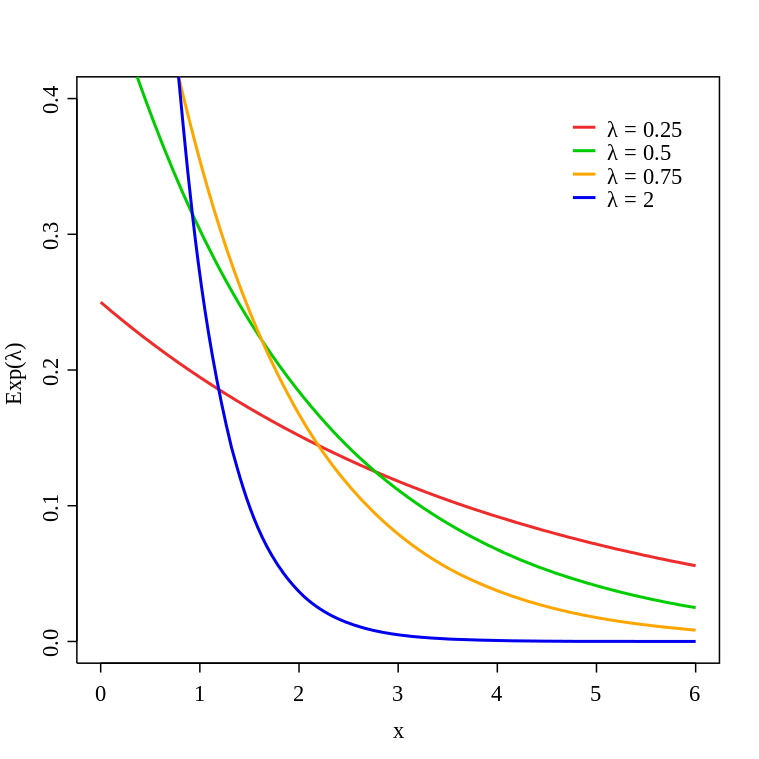
\includegraphics[width=0.39\textwidth]{./bilder/ExpDichteF}}\qquad
      \subfloat[Verteilungsfunktion]{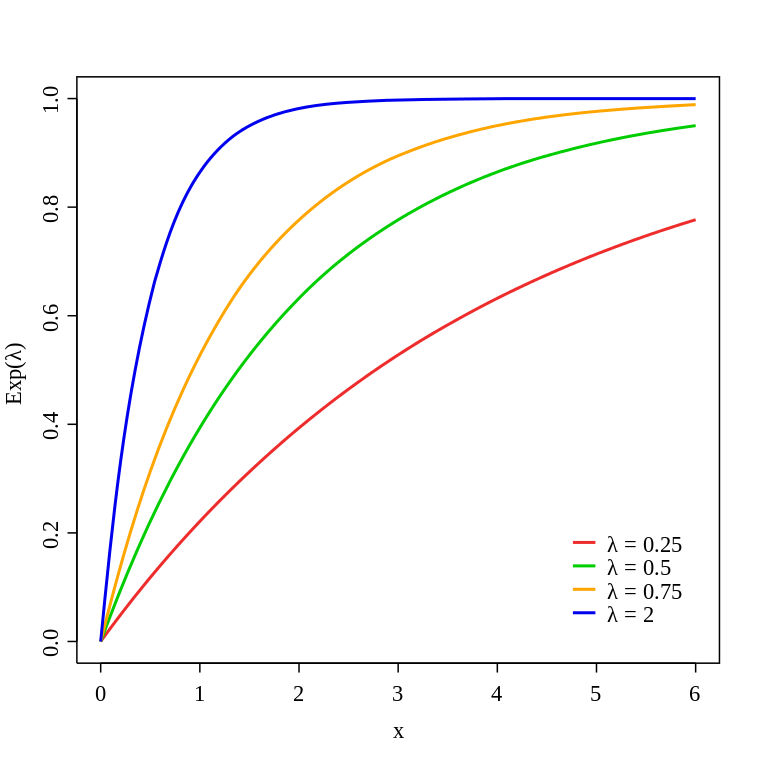
\includegraphics[width=0.39\textwidth]{./bilder/ExpVerteilungF}}
   \caption[Dichte- und Verteilungsfunktion der Exponentialverteilung]{Dichte- und Verteilungsfunktion der Exponentialverteilung}
\end{figure}

Sei $X \sim exp(\lambda)$ dann gilt:

\begin{enumerate}[label=(\roman{*})]
	\item Die Verteilungsfunktion von $X$ ist: 
	\begin{eqnarray*}
		F_X(x) = \int_{-\infty}^{x} f_{\lambda}(t) dt =
		\begin{cases}
			1-e^{-\lambda x} & \text{f�r } x\geq 0 \\ 	
			0 & \text{f�r } x<0 \\ 
		\end{cases}
	\end{eqnarray*}
	\item Der Erwartungswert ist:
	\begin{eqnarray*}
			\mathbb{E}(X) = \int_0^{\infty}\lambda xe^{-\lambda x} dx 
										= \left[-\frac{e^{-\lambda x}(\lambda x +1)}{\lambda}\right]^{\infty}_0
										= \frac{1}{\lambda}
	\end{eqnarray*}
	\item Die Varianz ist: 
	\begin{eqnarray*}
		Var(X) &=& \int_{0}^{\infty} \left(x-\frac{1}{\lambda}\right)^2 \lambda e^{-\lambda x} dx \\
					 &=& \int_{0}^{\infty} \left(x^2 -2x\frac{1}{\lambda} +  \frac{1}{\lambda ^2}\right) \lambda e^{-\lambda x} dx \\
					 &=& \lambda \int_{0}^{\infty} x^2e^{-\lambda x} dx- 2\int_{0}^{\infty}xe^{-\lambda x}dx +  \frac{1}{\lambda} \int_{0}^{\infty}e^{-\lambda x} dx \\
					 &=& \lambda \int_{0}^{\infty} x^2e^{-\lambda x} dx-\frac{2}{\lambda ^2} + \frac{1}{\lambda ^2} \\
					 &=& \lambda \big(\underbrace{\left[-\frac{1}{\lambda} x^2 e^{-\lambda x}\right]_0^{\infty}}_{\substack{0}} + \frac{2}{\lambda}\int_{0}^{\infty}xe^{-\lambda x}dx\big) - \frac{2}{\lambda ^2} \\
					 &=& \frac{2}{\lambda^2} - \frac{1}{\lambda^2} \\
					 &=& \frac{1}{\lambda^2}
	\end{eqnarray*}
	\item Die Exponentialverteilung ist ged�chtnislos (auch Nichtalterungseigenschaft genannt), d.h. f�r $X$ gilt:
	\begin{eqnarray*}
		\mathbb{P}(X> x+t\: | \: X > t) &=& \frac{\mathbb{P}(X> x+t, X > t)}{\mathbb{P}(X> t)} \\
					 &=& \frac{\mathbb{P}(X> x+t)}{\mathbb{P}(X> t)} \\
					 &=& \frac{e^{-\lambda (x+t)}}{e^{-\lambda t}} \\
					 &=& e^{-\lambda x} = \mathbb{P}(X> x)
	\end{eqnarray*}
\end{enumerate}

Die Exponentialverteilung hat die besondere Eigenschaft der Ged�chtnislosigkeit und es l�sst sich sogar zeigen, dass sie die einzige absolut stetige Verteilung\footnote{Im diskreten Fall ist dies die geometrische Verteilung.} mit dieser Eigenschaft ist:

\begin{lemmas} \label{expLemma} Sei X eine absolut stetige postive Zufallsvariable, dann gilt  $X \sim exp(\lambda)$ genau dann wenn f�r alle $x, t > 0$ gilt, dass
	\begin{eqnarray} \label{eq:ged}
		\mathbb{P}(X> x+t\: | \: X > t) = \mathbb{P}(X> x+t\: | \: X > t)
	\end{eqnarray}
\end{lemmas}

\textbf{Beweis:}
$\Rightarrow$ Sei $X \sim exp(\lambda)$ dann gilt:
	\begin{eqnarray*}
		\mathbb{P}(X> x+t\: | \: X > t) &=& \frac{\mathbb{P}(X> x+t, X > t)}{\mathbb{P}(X> t)} \\
					 &=& \frac{\mathbb{P}(X> x+t)}{\mathbb{P}(X> t)} \\
					 &=& \frac{e^{-\lambda (x+t)}}{e^{-\lambda t}} \\
					 &=& e^{-\lambda x} = \mathbb{P}(X> x)
	\end{eqnarray*}

$\Leftarrow$ Sei umgekehrt X eine absolut stetige Zufallsvariable, die die Gleichung \ref{eq:ged} erf�llt. Wir definieren $g(x) := \mathbb{P}(X > x)$. F�r $x, y > 0$ gilt:

\begin{eqnarray*}
	g(x + t) &=& \mathbb{P}(X > x + y) \\
					 &=& \mathbb{P}(X > x + y \: | \: X > y) \mathbb{P}(X > y) \\
					 &=& \mathbb{P}(X > x) \mathbb{P}(X > y) = g(x)g(y)
\end{eqnarray*}
Durch n-fache Anwendung folgt f�r alle $n \in \mathbb{N}$:

\begin{eqnarray*}
g(1) = g\big( \underbrace{\frac{1}{n} + ... + \frac{1}{n}}_{\substack{n-mal}} \big) = \left(g\big(\frac{1}{n}\big)\right)^n
\end{eqnarray*}
und somit insbesondere auch $g(\frac{1}{n}) = (g(1))^\frac{1}{n}$. Da X nur positive Werte annimmt, existiert ein $n \in \mathbb{N}$ mit $g(1/n) > 0$. Au�erdem existiert wegen $0 < g(1) \leq 1$, ein $\lambda \geq 0$ mit $g(1) = e^{-\lambda}$. F�r beliebige $p, q \in \mathbb{N}$ gilt 
\begin{eqnarray*}
	g(\frac{p}{q}) = g(\frac{1}{q})^p = g(1)^{\frac{p}{q}}
\end{eqnarray*}
und somit $g(r) = e^{-\lambda r}$ f�r alle $r \in \mathbb{Q}^+$. Aufgrund der Stetigkeit folgt daraus
\begin{eqnarray*}
	g(x) = e^{-\lambda x}
\end{eqnarray*}
\qed

\begin{defini}
Eine diskrete Zufallsvariable $X:\Omega\to \mathbb{N}$ hei�t \textbf{poissonverteilt zum Parameter $\lambda \in \mathbb{R}_{>0}$} (kurz $X\sim Poi(\lambda)$), wenn gilt:

\begin{eqnarray*}
	P_{\lambda}(k) := \mathbb{P}(X=k) = \frac{\lambda^k}{k!}e^{-\lambda}, k=0,1,2,...
\end{eqnarray*}
\end{defini}

Die Poisson-Verteilung hat folgende Eigenschaften:

\begin{enumerate}[label=(\roman{*})]
	\item Die Verteilungsfunktion der Poisson-Verteilung ist: 
	\begin{eqnarray*}
		F_{\lambda}(n) = \sum_{k=0}^{n} P_{\lambda}(k) = e^{-\lambda} \sum_{k=0}^{n} \frac{\lambda^k}{k!}
	\end{eqnarray*}
	\item Der Erwartungswert ist:
	\begin{eqnarray*}
			\mathbb{E}(X) &=& \sum_{k=0}^{\infty} k\frac{\lambda^k}{k!} e^{-\lambda}  
										=  0 + \sum_{k=1}^{\infty} k\frac{\lambda^k}{k!} e^{-\lambda} \\
										&=& \lambda e^{-\lambda} \sum_{k=1}^{\infty} \frac{\lambda^{k-1}}{(k-1)!} \\
										&=& \lambda e^{-\lambda} \sum_{i=0}^{\infty} \frac{\lambda^i}{i!} 
										= \lambda e^{-\lambda} e^{\lambda} 
										= \lambda
	\end{eqnarray*}
	
	Der Parameter $\lambda$ der Poisson-Verteilung kann also, als die erwartete Ereignish�ufigkeit pro Zeiteinheit interpretiert werden.
	
	\item Die Varianz ist: 
	\begin{eqnarray*}
		\mathbb{E}(X^2) &=& \sum_{k=0}^{\infty} k^2 \frac{\lambda^k}{k!} e^{-\lambda} \\
										&=& e^{-\lambda} \sum_{k=1}^{\infty} k \frac{\lambda^{k}}{(k-1)!} \\
										&=& e^{-\lambda} \sum_{k=1}^{\infty} \frac{((k-1)+1)\lambda^{k}}{(k-1)!} \\
										&=& e^{-\lambda} \sum_{k=2}^{\infty} \frac{\lambda^{k}}{(k-2)!} + e^{-\lambda} \sum_{k=1}^{\infty} \frac{\lambda^{k}}{(k-1)!} \\
										&=& \lambda^2 e^{-\lambda} \sum_{k=2}^{\infty} \frac{\lambda^{k-2}}{(k-2)!} + \lambda e^{-\lambda} \sum_{1}^{\infty} \frac{\lambda^{k-1}}{(k-1)!} \\
										&=& \lambda^2+\lambda \\ \\
						 Var(X) &=& \mathbb{E}(X^2) - \mathbb{E}(X)^2 = \lambda^2+\lambda - \lambda^2 = \lambda
	\end{eqnarray*}
	\item Seien $X_1$ und $X_2$ unabh�ngige poissonverteilte Zufallsvariablen mit $X_1\sim Poi(\lambda _1)$ und $X_2\sim Poi(\lambda _2)$, dann gilt f�r $X := X_1 + X_2 $:
		\begin{eqnarray*}
			\mathbb{P}(X=x) &=& \sum_{k=0}^{x} \mathbb{P}(X_1=k)\mathbb{P}(X_2=x-k) \\
											&=& e^{-\lambda_1}e^{-\lambda_2} \sum_{k=0}^{x} \frac{\lambda _{1} ^k}{k!} \frac{\lambda _{2} ^{x-k}}{(x-k)!} \\
											&=& \frac{e^{-(\lambda_1+\lambda_2)}}{x!} \sum_{k=0}^{x} \frac{x!}{k!(x-k)!}\lambda _{1}^k \lambda _{2}^{x-k} \\
											&=& e^{-(\lambda_1+\lambda_2)} \frac{(\lambda _{1} + \lambda _{2})^x}{x!} \\
				\Rightarrow  X &\sim & Poi(\lambda _1 + \lambda _2) 
		\end{eqnarray*}
		Das hei�t die Summe von poissonverteilten Zufallsvariablen ist wieder poissonverteilt.
	\end{enumerate}

Die Poisson-Verteilung hat au�erdem eine besondere Bedeutung, da sie unter den richtigen Voraussetzungen die Grenzverteilung der Binomialverteilung ist. Dieser Zusammenhang wird in folgendem Lemma verdeutlicht: \\

\begin{lemmas} Sei $X \sim B_{n,p}(k)$ eine binomialverteilte Zufallsgr��e. Wenn f�r $n \rightarrow \infty$ und $p \rightarrow 0$ gilt, dass der Erwartungswert $np$ gegen eine von $n$ unabh�ngige Konstante $\lambda$ konvergiert, dann konvergiert die Verteilungsfunktion von X gegen die Verteilungsfunktion einer, zum Parameter $\lambda$, poissonverteilten Zufallsgr��e.
\end{lemmas}

\textbf{Beweis:}
Wir zeigen, dass der Grenzwert $n\rightarrow \infty$ der Verteilungsfunktion einer binomialverteilten Zufallsvariable an der Stelle k, gegen den Wert einer poissonverteilten Zufallsvariablen an der Stelle k geht.

	\begin{eqnarray*}
		\lim_{\substack{n\rightarrow \infty\\p\rightarrow 0}} \mathbb{P}(X=k) &=& \lim_{\substack{n\rightarrow \infty\\p\rightarrow 0}}\binom{n}{k} p^k(1-p)^{n-k}\\
		&=& \lim_{\substack{n\rightarrow \infty\\p\rightarrow 0}} \frac{n!}{k!(n-k)!} \left(\frac{\lambda}{n}\right)^k \left(1-\frac{\lambda}{n}\right)^{n-k} \\
		&=& \frac{\lambda ^k}{k!} \lim_{\substack{n\rightarrow \infty\\p\rightarrow 0}} \underbrace{\left(\frac{n(n-1)(n-2)...(n-k+1)}{n^k}\right)}_{\rightarrow 1} \underbrace{\left( 1-\frac{\lambda}{n}\right)^{n}}_{\rightarrow e^{-\lambda}} \underbrace{\left(1-\frac{\lambda}{n}\right)^{-k}}_{\rightarrow 1} \\
		&=& \frac{\lambda ^k e^{-\lambda}}{k!}		
	\end{eqnarray*}
\qed
	
\section{Poisson Prozess}	
Ein weiteres Hilfsmittel, dass zur Modellierung verwendet wird, sind Stochastische Prozesse. Diese eignen sich sehr gut dazu geordnete zuf�llige Vorg�nge zu beschreiben.
Allgemein l�sst sich ein stochastischer Prozess wie folgt definieren.\\ 
	
\begin{defini}
Sei $(Z, \mathcal{Z})$ ein mit einer $\sigma$-Algebra versehener Raum, dann ist ein \textbf{Stochastischer Prozess} ist eine Familie von Zufallsvariablen $\{X_t, t\in T\}$ mit $X_t:\Omega\to Z$ und einer beliebigen nichtleeren Indexmenge $T$. Das hei�t $X$ ist eine Abbildung
\begin{eqnarray*}
	X:\Omega \times T \to Z, \; (\omega, t) \mapsto X_t(\omega)
\end{eqnarray*}
sodass $X_t: \omega \mapsto X_t(\omega)$ f�r alle  $t \in T$ eine messbare Abbildung ist. Z hei�t dann die \textbf{Zustandsmenge} und $(Z, \mathcal{Z})$ der \textbf{Zustandsraum}. Ein stochastische Prozess hei�t \textbf{zeitdiskret}, wenn $T$ abz�hlbar ist, z.B. $T = \mathbb{N}_0$. Ansonsten hei�t er \textbf{zeitstetig}. Analog hei�t ein Prozess mit diskreten Zustandsraum Z \textbf{wertdisktret} oder auch \textbf{Punktprozess}. 
\end{defini}

F�r unsere Zwecke reicht aus als Zustandsraum die reellen Zahlen mit der borelschen $\sigma$-Algebra zu betrachten. Da wir eine zeitliche Entwicklung untersuchen wollen, reicht es au�erdem wenn T eine Teilmenge der reellen Zahlen ist und als Zeit betrachtet wird. Das hei�t im folgenden sind die $\{X_t, t\geq 0\}$ reellwertige Zufallsvariablen. Mit dieser Einschr�nkung werden wir nun einige Eigenschaften vorstellen, die ein stochastischer Prozess haben kann.

\begin{enumerate}[label=(\roman{*})]
	\item Ein stochastische Prozess hei�t \textbf{station�r}, wenn f�r alle $n\geq 0, s\geq 0$, sowie alle $0\leq t_1 \leq t_2\leq ...\leq t_k$ und $x_1,x_2,...,x_k \in \mathbb{R}$ gilt:
		\begin{eqnarray*}
			\mathbb{P}(X_{t_1+s}\leq x_1, X_{t_2+s}\leq x_2,..., X_{t_k+s}\leq x_k)=\mathbb{P}(X_{t_1}\leq x_1, X_{t_2}\leq x_2,..., X_{t_k}\leq x_k)				
		\end{eqnarray*}
		Das hei�t, das zuf�llige Verhalten des Prozesses h�ngt nicht vom Zeitpunkt der Beobachtung ab.
	\item Analog besitzt ein stochastischer Prozess \textbf{station�re Zuw�chse}, wenn f�r alle $n\geq 0, s\geq 0$ und f�r alle $0\leq t_1 \leq t_2\leq ...\leq t_k\in T$ die Verteilung des Zufallsvektors $(X_{t_1+s}-X_{t_0+s},X_{t_2+s}-X_{t_1+s},...,X_{t_n+s}-X_{t_{n-1}+s})$ nicht von s abh�ngt.
	\item Ein stochastischer Prozess besitzt \textbf{Unabh�ngige Zuw�chse}, wenn die Zufallsvariablen $X_{t_0},X_{t_1}-X_{t_0},...,,X_{t_n}-X_{t_{n-1}}$ f�r alle n=1,2,... und $0\leq t_0<t_1<...<t_n$ unabh�ngig sind. 
\end{enumerate}

Stochastische Prozesse werden h�ufig dazu verwendet, die Eintrittszeitpunkte von zuf�lligen Ereignisses zu modellieren. Mit Blick auf die isolierten Ereignisse, interessiert uns allerdings eher wie viele Ereignisse in einem bestimmten Zeitraum eintreten werden. Die f�hrt zu der folgenden Definition.

\begin{defini} \label{def:zaehlPro}
Sei $T_1, T_2, ... : \Omega \rightarrow \mathbb{R}, \omega \rightarrow [0, \infty)$ eine Folge von unabh�ngig und identisch verteilten Zufallsvariablen und $S_n := T_1+...+T_n$ f�r alle $n\in \mathbb{N}$, dann ist $N := \{N_t, t\geq 0\}$ mit
\begin{eqnarray*}
		N_t = \sum_{k=1}^{\infty} \mathds{1}(S_k\leq t)
\end{eqnarray*}
ein stochastischer Prozess und wird als Z�hlprozess bezeichnet. 
\end{defini}

Betrachten wir wieder unser Beispiel mit den Abfahrtszeitpunkten von Bussen, dann k�nnen wir die $T_n$ als Wartezeit auf den n�chsten Bus auffassen, nachdem gerade einer abgefahren ist. Die $S_n$ hingegen sind die Zeitpunkte zu denen jeweils ein Bus f�hrt. Deshalb ist naheliegend die $T_n$ als \textbf{Zwischenankunftszeiten} zu bezeichnen und die $S_n$ als $n$-te \textbf{Sprungzeit}. Prozesse dieser Art werden z.B. auch in der Zuverl�ssigkeitstheorie eingesetzt, um die Ausf�lle einer Komponente in einem bestimmten Zeitraum zu z�hlen. Der Zusammenhang zur vorher eingef�hrten Poisson-Verteilung wird im Folgenden deutlich.

\begin{defini} \label{def:poiPro}
Ein Z�hlprozess $\{N_t, t\geq 0\}$ mit exponentialverteilten Zwischenankunftszeiten $T_n \sim exp(\lambda)$ hei�t \textbf{homogener Poisson-Prozess mit der Intensit�t $\lambda$}.  
\end{defini}

In dem nachfolgendem Theorem werden die wichtigsten Eigenschaften und �quivalenten Definitionen des Poisson-Prozesses deutlich. Vorher ben�tigen wir jedoch folgende Definition: \\

\begin{defini}
Seien $X_1, X_2,..., X_n$, mit $n\in \mathbb{N}$ Zufallsvariablen, dann bezeichnen wir die geordneten Variablen $X_{1:n} \leq X_{2:n} \leq ... \leq X_{n:n}$ als die \textbf{Ordnungsstatistik} der Variablen $\{X_i: 1 \leq i \leq n\}$.
\end{defini}

\begin{satz}
Seien $X_1, X_2,..., X_n$, mit $n\in \mathbb{N}$, unabh�ngige und identisch verteilte Zufallsvariablen mit Dichte $f$ und sei $X_{1:n} \leq X_{2:n} \leq ... \leq X_{n:n}$ die entsprechende Ordnungsstatistik. Dann gilt f�r die gemeinsame Dichte:
\begin{eqnarray}\label{eq:ordnungsstatistik}
f_{X_{1:n},X_{2:n},...,X_{n:n}}(t_1,t_2...,t_n)=
		\begin{cases}
			n!f(t_1)f(t_2)...f(t_n) & \text{falls } t_1\leq t_2\leq ... \leq t_n \\ 	
			0 & \text{sonst} \\ 
		\end{cases}
\end{eqnarray}
\end{satz} 

\textbf{Beweis:} 
Da aufgrund der Definition der Ordnungsstatistik die Werte aufsteigend geordnet sind, ist die Dichte gleich 0, wenn die Bedingung $t_1\leq t_2\leq ... \leq t_n$ nicht erf�llt ist. Sei nun diese Bedingung erf�llt. Dann existieren genau $n!$ M�glichkeiten die Zufallsvariablen $X_1, X_2,..., X_n$ anzuordnen. Zum Beispiel gilt f�r $n=2$, dass $\{X_{1:2} = t_1, X_{2:2} = t_2\}$ genau dann Eintritt wenn entweder $\{X_1 = t_1, X_2 = t_2\}$ oder $\{X_2 = t_1, X_1 = t_2\}$ eintritt. Diese M�glichkeiten unterscheiden sich nur durch Permutation und besitzen somit die gleiche Dichte. Deshalb reicht es aus nur eine M�glichkeit zu betrachtet und das Ergebnis anschlie�end mit der Anzahl der m�glichen Permutationen $n!$ zu multiplizieren. Es gilt f�r die einfachste M�glichkeit
\begin{eqnarray*}
f_{X_1,X_2,...,X_n}(t_1,t_2...,t_n)=f(t_1)f(t_2)...f(t_n)
\end{eqnarray*}
da die Zufallsvariablen $X_1, X_2,..., X_n$ unabh�ngig voneinander sind. Nach Multiplikation mit $n!$ ist erh�lt man \ref{eq:ordnungsstatistik}.
\qed \\

\begin{theorem} \label{th:poiPro} Die folgenden Aussagen sind �quivalent\footnote{Quelle siehe: \url{http://www.mathematik.uni-ulm.de/stochastik/lehre/ss05/wt/skript/node15.html}}:
\begin{enumerate}[label=(\roman{*})]
	\item $\{N_t, t\geq 0\}$ ist ein Poisson-Prozess mit der Intensit�t $\lambda$
	\item Die Zufallsvariablen $N_t$ sind poissonverteilt zum Parameter $\lambda t$ f�r alle $t\geq 0$. \\
	
	Unter der Bedingung $\{N_t = n\}$, hat f�r beliebige $n=1,2,...$ der Zufallsvektor $(S_1, S_2,...,S_n)$, die gleiche Verteilung wie die Ordnungsstatistik von n unabh�ngigen, in $[0,t]$ gleichverteilten Zufallsvariablen.
	\item Der stochastische Prozess $\{N_t, t\geq 0\}$ hat unabh�ngige Zuw�chse und es gilt $\mathbb{E}(N_1) = \lambda$. \\
	
	Unter der Bedingung $\{N_t = n\}$, hat f�r beliebige $n=1,2,...$ der Zufallsvektor $(S_1, S_2,...,S_n)$, die gleiche Verteilung wie die Ordnungsstatistik von n unabh�ngigen, in $[0,t]$ gleichverteilten Zufallsvariablen.
	\item Der stochastische Prozess $\{N_t, t\geq 0\}$ hat unabh�ngige und station�re Zuw�chse und es gilt f�r $h \rightarrow 0$:
	\begin{eqnarray*}
		\mathbb{P}(N_h =0) &=& 1-\lambda h + o(h) \text{, und} \\
		\mathbb{P}(N_h =1) &=& \lambda h + o(h)\
	\end{eqnarray*}
	\item Der stochastische Prozess $\{N_t, t\geq 0\}$ hat unabh�ngige und station�re Zuw�chse. Au�erdem gilt f�r jedes $t\geq 0$ das $N_t \sim Poi(\lambda t)$.
\end{enumerate}
\end{theorem}

\textbf{Beweis:} 
\begin{itemize}
\item $(i) \Rightarrow (ii)$:
Seien ${T_i}_i\in \mathbb{N}$	die Zwischenankunftszeiten des Poisson-Prozesses $\{N_t, t\geq 0\}$, dann folgt, dass $S_n=\sum_{i=1}^n T_i$ eine Summe von $n$ unabh�ngigen und zum Parameter $\lambda$ exponentialverteilten Zufallsvariablen ist. 	Nach \ref{lem:gamma} gilt also $S_n \sim \gamma_{\lambda, n}$. Hieraus folgt $\mathbb{P}(N_t = 0) = \mathbb{P}(S_1 > t) = e^{-\lambda t}$ und damit gilt:

\begin{eqnarray*}	 
	\mathbb{P}(N_t = n) &=&\mathbb{P}(N_t \geq n) - \mathbb{P}(N_t \geq n+1) \\	 
				&=&\mathbb{P}(S_n \leq t)- \mathbb{P}(S_{n+1} \leq t) \\
				&=&\int_0^t \frac{\lambda^n v^{n-1}}{(n-1)!} e^{-\lambda v} \mathrm{d}v - \int_0^t \frac{\lambda^{n+1}v^n}{n!} e^{-\lambda v} \mathrm{d}v	 \\
				&=&\int_0^t \frac{\mathrm{d}}{\mathrm{d}v} \left(\frac{(\lambda v)^n}{n!} e^{-\lambda v}\right) \mathrm{d}v \\
				&=&\frac{(\lambda t)^n}{n!} e^{-\lambda t}
\end{eqnarray*}

Dies gilt f�r jedes $n\geq 1$, und damit folgt, dass $N_t \sim Poi(\lambda t)$. Dies ist der erste Teil von $(ii)$ und f�r den zweiten Teil betrachten wir die gemeinsame Dichte $f_{S_1,...,S_{n+1}}(t_1,...,t_{n+1})$ von $S_1,...,S_{n+1}$. F�r beliebige $t_0=0 \leq t_1 \leq ... \leq t_n \leq t_{n+1}$ gilt aufgrund des Transformationssatzen (vgl. \ref{sa:trafo})

\begin{eqnarray*}	 
	f_{S_1,...,S_{n+1}}(t_1,...,t_{n+1}) &=& f_{T_1,T_2,...,T_{n+1}}(t_1,t_2-t_1,...,t_{n+1}-t_n) * |det(DA)| \\
						&=& \prod_{k=1}^{n+1} \lambda e^{-\lambda(t_k-t_{k-1})} = \lambda^{n+1}e^{-\lambda t_{n+1}}
\end{eqnarray*}

und 0 sonst. Dabei ist A die Transformation $t_i \mapsto t_i - t_{i-1}$ und damit gilt $|det(DA)| = 1$. Somit gilt unter der Bedingung $N_t=n$ und $0 \leq t_1 \leq ... \leq t_n \leq t$ f�r die gemeinsame bedingte Dichte

\begin{eqnarray*}	 
	f_{S_1,...,S_n}(t_1,...,t_n\: | \:N_t=n) &=& f_{S_1,...,S_n}(t_1,...,t_n\: | \:S_1 \leq t,...,S_n\leq t, S_{n+1} > t) \\
																						&=& \frac{\int_t^{\infty} \lambda^{n+1} e^{-\lambda x_{n+1}} dx_{n+1}}
																						{\int_0^t \int_{x_1}^t .. .\int_{x_{n-1}}^t \int_t^{\infty} \lambda^{n+1} e^{-\lambda x_{n+1}} dx_{n+1}...dx_1} \\
																						&=& \frac{n!}{t^n}
\end{eqnarray*}

und $f_{S_1,...,S_n}(t_1,...,t_n\: | \:N_t=n) = 0$ sonst. Nach \ref{eq:ordnungsstatistik} ist dies die Dichte der Ordnungsstatistik von n unabh�ngigen in[0,t] gleichverteilten Zufallsvariablen und damit der zweite Teil dieses Beweisschritts. 

\item $(ii) \Rightarrow (iii)$: 

Aufgrund von $(ii)$ gilt $N_t \sim Poi(\lambda t)$ und damit ist $\mathbb{E} N_1 = \lambda$. Nun zeigen wir, dass der Prozess unabh�ngige Zuw�chse hat. Dazu seien $x_1,...,x_n \in \mathbb{N}$ und $t_0=0 \leq t_1 \leq ... \leq t_n$, dann gilt f�r $x=x_1+...+x_n$. Es gilt f�r die Zuw�chse

\begin{eqnarray*}	 
	\mathbb{P}(N_{t_1}-N_{t_0}=x_1) &=& \mathbb{P}\big(\sum_{k=1}^{\infty} \mathds{1}_{\{S_k \leq t_1\}} - \mathds{1}_{\{S_k \leq t_0\}} = x_1\big) \\
																	&=& \mathbb{P}\big(\sum_{k=1}^{\infty} \mathds{1}_{\{S_k \in (t_0, t_1]\}} = x_1\big)\\
																	&=& \mathbb{P}(S_1 \in (t_0, t_1],...,S_{x_1} \in (t_0, t_1])
\end{eqnarray*}

Damit k�nnen, unter Ausnutzung der Nebenbedingung, schreiben
\begin{eqnarray*}	 
	&& \mathbb{P}(N_{t_1}-N_{t_0} = x_1,...,N_{t_n}-N_{t_{n-1}} = x_n \: | \: N_{t_n}=x)\\
	&=& \mathbb{P}(S_1 \in (t_0, t_1],...S_{x_1} \in (t_0, t_1],...,S_{x-x_n+1} \in (t_{n-1}, t_n],...,S_x \in (t_{n-1}, t_n] \: | \: N_{t_n}=x)\\
	&=& \int_{(t_0,t_1]^{x_1}\times...\times(t_{n-1},t_n]^{x_n}} f_{S_1,...,S_x}(y_1,...,y_x \: | \:N_{t_n}=x) dy_x...dy_1 \\
	&=& \int_{(t_0,t_1]^{x_1}\times...\times(t_{n-1},t_n]^{x_n}} \frac{x!}{t_n^x} dy_x...dy_1 \\
	&=& \frac{x!}{t_n^x} \int_{(t_0,t_1]^{x_1}} \mathds{1}_{\{y_1\leq y_2\}}...\mathds{1}_{\{y_{x_1-1}\leq y_{x_1}\}}dy_{x_1}...dy_1 *...\\
	&&*\int_{(t_{n-1},t_n]^{x_n}} \mathds{1}_{\{y_{x-x_n+1}\leq y_{x-x_n+2}\}}...\mathds{1}_{\{y_{x-1}\leq y_x\}}dy_x...dy_{x-x_n+1}\\
	&=& \frac{x!}{t_n^x} \int_{t_0}^{t_1}\int_{y_1}^{t_1}...\int_{y_{x_1-1}}^{t_1} dy_{x_1}...dy_1 * ... * \int_{t_{n-1}}^{t_n}\int_{y_{x-x_n+1}}^{t_n}...\int_{y_{x-1}}^{t_n} dy_x...dy_{x-x_n+1}
\end{eqnarray*}

Nach Nebenrechnung \ref{nr:integral1} k�nnen wir die Integrale direkt angeben und damit ist
\begin{eqnarray*}	 
	\mathbb{P}(N_{t_1}-N_{t_0} = x_1,...,N_{t_n}-N_{t_{n-1}} = x_n \: | \: N_{t_n}=x) &=& \frac{x!}{t_n^x} \prod_{k=1}^n \frac{(t_k-t_{k-1})^{x_k}}{x_k!} \\
																																										&=& \frac{x!}{x_1!x_2!...x_n!} \prod_{k=1}^n \big(\frac{t_k-t_{k-1}}{t_n}\big)^{x_k}.
\end{eqnarray*}

Deshalb gilt

\begin{eqnarray*}	 
	\mathbb{P}(\bigcap_{k=1}^n\{N_{t_k}-N_{t_{k-1}}=x_k\})&=& \mathbb{P}(N_{t_1}-N_{t_0} = x_1,...,N_{t_n}-N_{t_{n-1}} = x_n)\\
	&=& \mathbb{P}(N_{t_1}-N_{t_0} = x_1,...,N_{t_n}-N_{t_{n-1}} = x_n \: | \: N_{t_n}=x)\mathbb{P}(N_{t_n}=x)\\
	&=& \frac{(\lambda t_n)^x}{x!}e^{-\lambda t_n} \frac{x!}{x_1!...x_n!} \prod_{k=1}^n \left(\frac{t_k-t_{k-1}}{t_n}\right)^{x_k} \\
	&=& \prod_{k=1}^n \frac{(\lambda (t_k-t_{k-1}))^{x_k}}{x_k!} e^{-\lambda (t_k - t_{k-1})}
\end{eqnarray*}

und damit hat der Z�hlprozess ${N_t}$ unabh�ngige Zuw�chse.

\item $(iii) \Rightarrow (iv)$: 

Aus $(iii)$ folgt, dass der Zufallsvektor $(S_1,...,S_m)$, unter der Bedingung $N(t_n + h) = m$, die gleiche Verteilung hat, wie die Ordnungstatistik vom m unabh�ngigen in $[0, t_n + h]$ gleichverteilten Zufallsvariablen hat. Deshalb gilt f�r beliebige $x_1,...,x_n \in \mathbb{N}$ mit $x_1+...+x_n =m$, $t_0=0 \leq t_1 \leq ... \leq t_n$ und $h>0$ 

\begin{eqnarray*}	 
	&& \mathbb{P}(\bigcap_{k=1}^n\{N_{t_k+h}-N_{t_{k-1}+h}=x_k\}\: | \:N_{t_n+h}=m)\\
	&=& \frac{x!}{x_1!x_2!...x_n!} \prod_{k=1}^n \big(\frac{t_k+h-t_{k-1}-h}{t_n+h}\big)^{x_k} \\
	&=& \frac{x!}{x_1!x_2!...x_n!} \prod_{k=1}^n \big(\frac{t_k-t_{k-1}}{t_n+h}\big)^{x_k} \\
	&=& \mathbb{P}(\bigcap_{k=1}^n\{N_{t_k}-N_{t_{k-1}}=x_k\}\: | \:N_{t_n+h}=m)
\end{eqnarray*}

Aufgrund der Formel der totalen Wahrscheinlichkeit folgt damit, dass ${N_t}$ station�re Zuw�chse besitzt. Die Gleichverteilungseigenschaft aus $(iii)$ liefert au�erdem f�r $0<h<1$

\begin{eqnarray*}	 
	\mathbb{P}(N_h=0) &=& \sum_{k=0}^\infty \mathbb{P}(N_h=0,N_1-N_h=k)\\
		&=& \sum_{k=0}^\infty \mathbb{P}(N_1=k)\mathbb{P}(N_1-N_h=k\: | \:N_1=k)\\
		&=& \sum_{k=0}^\infty \mathbb{P}(N_1=k)(1-h)^k
\end{eqnarray*}

und somit gilt

\begin{eqnarray*}	 
	\frac{1}{h}(1-\mathbb{P}(N_h=0)) &=& \frac{1}{h}\left(1-\sum_{k=0}^\infty \mathbb{P}(N_1=k)(1-h)^k\right)\\
		&=& \sum_{k=1}^\infty \mathbb{P}(N_1=k) \frac{1-(1-h)^k}{h}
\end{eqnarray*}

Da $(1-h)^k\geq1-kh$ f�r beliebige $0<h<1$ und $k=1,2,...$ gilt, folgt, dass die Funktionen $g_h(k)=\frac{1-(1-h^k)}{h}$ die gemeinsame Schranke $g(k)=k$ besitzen.
Diese Schranke ist integrierbar, da gilt

\begin{eqnarray*}	 
	\sum_{k=1}^\infty k\mathbb{P}(N_1=k) = \mathbb{E}(N_1) = \lambda < \infty .
\end{eqnarray*}

Durch die Vertauschung von Summe und Grenzwert, ergibt sich

\begin{eqnarray*}	 
	\lim_{h \rightarrow 0} \frac{1}{h} \mathbb{P}(N_h>0) = \lambda
\end{eqnarray*}

und damit der erste Grenzwert von $(iv)$. Analog dazu gilt

\begin{eqnarray*}	 
	\lim_{h \rightarrow 0} \frac{1}{h} \mathbb{P}(N_h=1) = \lim_{h \rightarrow 0} \sum_{k=1}^\infty \mathbb{P}(N_1=k)k(1-h)^{k-1} = \lambda
\end{eqnarray*}

was �quivalent zur zweiten Bedingung in $(iv)$ ist.

\item $(iv) \Rightarrow (v)$: 

Sei $ p_n(t) := \mathbb{P}(N_t=n)$ mit $n\in \mathbb{N}$ und $t\geq0$, dann gilt f�r $h>0$

\begin{eqnarray} \label{eq:th1a}
	p_0(t+h)&=& \mathbb{P}(N_t=0,N_{t+h}-N_t=0) \\
					&=& \mathbb{P}(N_t=0) \mathbb{P}(N_{t+h}-N_t=0) \\
					&=& \mathbb{P}(N_t=0) \mathbb{P}(N_h=0) \\
					&=& p_0(t)(1-\lambda h + o(h))
\end{eqnarray}

und f�r $t\geq h>0$

\begin{eqnarray} \label{eq:th1b} 
	p_0(t)=p_0(t-h)(1-\lambda h + o(h))
\end{eqnarray}

Damit ist $p_0(t)$ stetig in $(0,\infty)$ und rechtsstetig im Punkt $t=0$. Da $p_0(t-h)=p_0(t)+o(1)$ folgt aus \ref{eq:th1a} und \ref{eq:th1b}, dass f�r beliebige $h\geq -t$ gilt

\begin{eqnarray*}	 
	\frac{p_0(t+h)-p_0(t)}{h}=-\lambda p_0(t) + o(1)
\end{eqnarray*}

Das zeigt das $p_0(t)$ differenzierbar ist und es ergibt sich f�r t>0 folgende Differenzialgleichung

\begin{eqnarray*}	 
	p_0'(t)=-\lambda p_0(t).
\end{eqnarray*}

Durch die Randbedingung $p_0(0) = \mathbb{P}(N_0=0) = 1$ ist die eindeutig bestimmte L�sung 

\begin{eqnarray*}	 
	p_0(t)= e^{-\lambda t} , t\geq 0.
\end{eqnarray*} 

F�r beliebige $n\in \mathbb{N}$ gilt 

\begin{eqnarray*}	 
	p_n(t)= \frac{(\lambda t)^n}{n!}e^{-\lambda t} , t\geq 0.
\end{eqnarray*} 

Dies l�sst sich analog zum vorherigen Fall zeigen und durch vollst�ndige Induktion nach n folgt $(v)$.

\item $(v) \Rightarrow (i)$:
 
Sei $ b_0 = 0 \le a_1 < b_1 \leq ...\leq a_n < b_n$, dann gilt

\begin{eqnarray*}	 
	&& \mathbb{P}\left(\bigcap_{k=1}^n\{ a_k < S_k \leq b_k\}\right)	= \\
	&& \mathbb{P}\left(\bigcap_{k=1}^{n-1}\{N_{a_k} -N_{b_{k-1}} = 0, N_{b_k} - N_{a_k} = 1\} \cap \{N_{a_n} - N_{b_{n-1}} = 0, N_{b_n} - N_{a_n} \geq 1\}\right).
\end{eqnarray*} 

Nach $(v)$ ist der stochastische Prozess station�r und die $N_t \sim Poi(\lambda t=)$ deshalb gilt
\begin{eqnarray*}	 
	\mathbb{P}(N_{a_k} -N_{b_{k-1}} = 0) = \mathbb{P}(N_{a_k-b_{k-1}} = 0) = e^{-\lambda (a_k-b_{k-1})}
\end{eqnarray*} 

und

\begin{eqnarray*}	 
	\mathbb{P}(N_{b_k} -N_{a_k} = 1) = \mathbb{P}(N_{b_k-a_k} = 1) = \lambda (b_k-a_k)e^{-\lambda (b_k-a_k)}.
\end{eqnarray*} 

Da die Intervalle $\{(b_{k-1},a_k)\}_{1\leq k \leq n}$ und $\{(a_k, b_k)\}_{1\leq k \leq n}$ disjunkt sind und der Prozess unabh�ngige Zuw�chse hat, gilt

\begin{eqnarray*}
	&& \mathbb{P}\left(\bigcap_{k=1}^n\{ a_k < S_k \leq b_k\}\right) \\
	&=& e^{-\lambda(a_n - b_{n-1})} (1 - e^{-\lambda(b_n - a_n)}) \prod_{k=1}^{n-1} e^{-\lambda(a_k - b_{k-1})} \lambda (b_k -a_k) e^{-\lambda(b_k - a_k)} \\
	&=& (e^{-\lambda a_n} - e^{-\lambda b_n})\lambda^{n-1} \prod_{k=1}^{n-1} (b_k - a_k) \\
	&=& \int_{a_1}^{b_1}...\int_{a_n}^{b_n} \lambda^n e^{-\lambda y_n} dy_n...dy_1 \\
	&=& \int_{a_1}^{b_1}\int_{a_2 - x_1}^{b_2 - x_1}...\int_{a_n-x_1-...-x_{n-1}}^{b_n-x_1-...-x_{n-1}} \lambda^n e^{-\lambda(x_1 +...+x_n)} dx_n...dx_1.
\end{eqnarray*}

Dabei wurde im letzten Schritt wieder der Transformationssatz angewendet. Die gemeinsame Dichte von  $ S_1, S_2 - S_1, ...,S_n - S_{n-1}$ ist somit gegeben durch

\begin{eqnarray*}
	f_{T_1,..T_n}=f_{S_1,S_2-S_1,...,S_n-S_{n-1}}(x_1,...,x_n) = \lambda^n e^{-\lambda(x_1 + ... +x_n)}.
\end{eqnarray*}

Dies bedeutet, dass die Zufallsvariablen  $T_1, T_2...,T_n$ unabh�ngig und exponentialverteilt zum Parameter $\lambda$ sind, d.h., $ \{N_t\}$ ist ein Poisson-Prozess mit der Intensit�t $ \lambda$. 

\end{itemize}
\qed

Die folgende sehr n�tzliche Eigenschaft ist bereits von der Poisson-Verteilung bekannt:

\begin{lemmas} \label{lem:aufteilungPP}
Die �berlagerung von zwei unabh�ngigen Poisson-Prozessen $\{N_t^1, t\geq 0\}$ und $\{N_t^2, t\geq 0\}$  mit der Intensit�t $\lambda _1$ bzw. $\lambda _2$ ist wieder ein Poisson-Prozess mit Intensit�t $\lambda = \lambda _1+\lambda _2$.
\end{lemmas}
\textbf{Beweis:} 
Im vorangegangen Theorem hab wir gezeigt, dass f�r einen Poisson-Prozess $\{N_t, t\geq 0\}$ gilt $N_t \sim Poi(\lambda t)$. Da $\{N_t^1, t\geq 0\}$ und $\{N_t^2, t\geq 0\}$ unabh�ngig sind gilt f�r die Summe $N_t^1 + N_t^2 \sim Poi((\lambda _1 + \lambda _2)t)$. Damit ist die �berlagerung der beiden Poisson-Prozesse wieder ein Poisson-Prozess mit Intensit�t $\lambda = \lambda _1+\lambda _2$.
\qed \\

Ein interessantes Ph�nomen ist zu beobachten, wenn bei sich bei einem Poisson-Prozess die Zeit bis zum n�chsten Ereignis, zu einem beliebigen Zeitpunkt, betrachtet.
\begin{defini} 
Sei $\{N_t, t\geq 0\}$ ein Z�hlprozess mit Zwischenankunftszeiten $T_1, T_2, ...$ und Sprungzeiten $\{S_n, n\in \mathbb{N}\}$. Weiterhin bezeichne $W_t$ Wartezeiten bis zum n�chsten Sprung und $V_t$ die Zeit seit dem letzten Sprung. Des Weiteren bezeichne $T_{N_{t+1}}$ die $t$ enthaltende Zwischenankunftszeit und Analog sind $S_{N_t}$ bzw. $S_{N_{t+1}}$ die letzte Sprungzeit vor $t$ bzw. die n�chste nach $t$. Dann gilt:
\begin{eqnarray*}
	V_t+W_t &=& T_{N_{t+1}} = S_{N_{t+1}}- S_{N_t} \\
	V_t &=& t-S_{N_t} \\
	W_t &=& S_{N_{t+1}}-t
\end{eqnarray*}
\end{defini}

\begin{lemmas}\label{lem:wartezeit}
Sei $\{N_t, t\geq 0\}$ homogener Poisson-Prozess mit Intensit�t $\lambda$. Dann ist $W_t \sim exp(\lambda)$ f�r alle $t > 0$.
\end{lemmas}

\textbf{Beweis:} 
Da die Zwischenankunftszeiten eines Poisson-Prozesses exponentialverteilt sind, folgt der Beweis direkt aus der Ged�chtnislosigkeit der Exponentialverteilung:
\begin{eqnarray*}
	\mathbb{P}(W_t \leq s) &=& \mathbb{P}(T_{N_{t+1}} \leq V_t+s) \\
	&=& \mathbb{P}(T_{N_{t+1}} \leq V_t+s \: | \: T_{N_{t+1}} > V_t) \\
	&=& \mathbb{P}(T_{N_{t+1}} \leq s) =1-e^{-\lambda s}
\end{eqnarray*}
D.h. die Wartezeit zum Zeitpunkt t ist genauso verteilt wie die Zwischenankunftszeiten und damit unabh�ngig davon, wie viel Zeit bereits seit dem letzten Ereignis vergangen ist.
\qed \\

F�r unser Beispiel mit den Bussen bedeutet das, dass egal zu welchem Zeitpunkt wir zur Haltestelle gehen, die Wartezeit auf den n�chsten Bus hat immer die gleiche Verteilung. Nachdem wir ausf�hrlich den Poisson-Prozess betrachtet haben, wollen wir nun einen stochastischen Prozess einf�hren, der h�ufig in der Risikotheorie f�r die Modellierung von Schadensh�hen verwendet wird.

\begin{defini}
Sei $\{N_t, t\geq 0\}$ ein homogener Poisson-Prozess mit Intensit�t $\lambda$ und seien $X_1, X_2, ...$ unabh�ngige, nichtnegative und identisch verteilte Zufallsvariablen. Dann hei�t der Prozess
\begin{eqnarray*}
	Y_t = \sum_{i=1}^{N_t} X_i
\end{eqnarray*}
\textbf{zusammengesetzter Poisson-Prozess}.
\end{defini}

Der Erwartungswert eines zusammengesetzten Poisson-Prozesses l�sst sich einfach bestimmen:
\begin{lemmas}
Sei $Y_t = \sum_{i=1}^{N_t} X_i$ ein zusammengesetzter Poisson-Prozess und $\mathbb{E}(X_i) = \mu$, dann gilt f�r alle $t\geq 0$
\begin{eqnarray*}
	\mathbb{E}(Y_t) = \mu \lambda t
\end{eqnarray*}
\end{lemmas}

\textbf{Beweis:} 
Da die $X_i$ unabh�ngig sind, gilt nach der Satz der totalen Erwartung
\begin{eqnarray*}
	\mathbb{E}(Y_t) &=& \mathbb{E}\left(\sum_{i=1}^{N_t} X_i\right) \\
	&=& \sum_{n=1}^{\infty} \mathbb{E}\left(\sum_{i=1}^{N_t} X_i \:|\: N_t=n\right)\mathbb{P}(N_t = n) \\
	&=& \sum_{n=1}^{\infty} \mathbb{E}\left(\sum_{i=1}^{n} X_i\right)\mathbb{P}(N_t = n) \\
	&=& \sum_{n=1}^{\infty} \mu n *\mathbb{P}(N_t = n) \\
	&=& \mu \mathbb{E}(N_t) = \mu \lambda t
\end{eqnarray*}
\qed \\
	
\section{Markov-Kette}\label{sec:markov}
Als n�chstes werden wir eine weitere wichtige Klasse an stochastischen Prozessen vorstellen. Dieser Abschnitt basiert zum Gro�teil auf dem Skript von Professor Wolfgang K�nig, "`Wahrscheinlichkeitstheorie I und II"'\footnote{Aktuelle Version unter \url{http://www.wias-berlin.de/people/koenig/www/Skripte.html} (Stand: 16.01.2015)}.

\begin{defini} 
Ein Stochastischer Prozess $\{X_t, t >0\}$ aus $I$-wertigen Zufallsvariablen, besitzt die \textbf{Markoveigenschaft}, wenn f�r $t_0, t_1,...t_n,t_{n+1} \in T$ und alle $i_0,i_1,...,i_{n+1} \in I$ gilt:
\begin{eqnarray}
\label{eq:markov}
	\mathbb{P}(X_{t_{n+1}}=i_{n+1}\: | \:X_{t_n}=i_n,X_{t_{n-1}}=i_{n-1},...,X_{t_0}=i_0) = \mathbb{P}(X_{t_{n+1}}=i_{n+1}\: | \:X_{t_n}=i_n)
\end{eqnarray}

Ein diskreter stochastischer Prozess der \ref{eq:markov} erf�llt hei�t \textbf{Markov-Kette}. Die \textbf{Startverteilung} der Markov-Kette ist definiert durch $v(i) := \mathbb{P}(X_0 = i)$ und die Wahrscheinlichkeiten $\mathbb{P}(X_{t_{n+1}}=i_{n+1}\: | \:X_{t_n}=i_n) =: p_{i_n , i_{n+1}}$ werden als \textbf{�bergangswahrscheinlichkeiten} bezeichnet. Die Matrix $P = (p_{i,j})_{i, j \in I}$ die sich aus den �bergangswahrscheinlichkeiten ergibt hei�t \textbf{�bergangsmatrix}.
\end{defini}

Der n�chste Zustand einer Markov-Kette h�ngt also immer nur von dem aktuellen Zustand ab. D.h. die Kette wird durch die �bergangswahrscheinlichkeiten charakterisiert. Deshalb hat die �bergangsmatrix auch eine besondere Struktur. Im folgenden betrachten wir lediglich den stetigen Fall, d.h die Zustandsmenge $I$ ist eine nichtleere, endliche oder h�chstens abz�hlbar unendliche Menge und die Indexmenge T ist eine Teilmenge von $\mathbb{N}$. 

\begin{defini} Eine Matrix $P = (p_{i,j})$ hei�t \textbf{stochastisch}, falls f�r alle $i, j \in I$ (Indexmenge) gilt  $p_{i,j} \in [0, 1]$ und $\sum_{j \in I} p_{i,j} = 1$.
\end{defini}

Die �bergangsmatrix ist also eine stochastische Matrix, welche f�r jeden Zustand eine Zeile besitzt, in der die m�glichen �berg�nge des entsprechenden Zustands, in andere Zust�nde und die dazugeh�rigen Wahrscheinlichkeiten angegeben wird. 

\begin{lemmas}
Sei $\{X_n, n\in \mathbb{N}\}$ eine Folge von $I$-wertigen Zufallsgr��en, $v$ eine Verteilung auf $I$ und $P$ eine stochastische Matrix, dann ist $\{X_t,n\in \mathbb{N}\}$ genau dann eine Markov-Kette mit �bergangsmatrix $P$ und Startverteilung $v$, wenn f�r alle $n\in\mathbb{N}$ und alle $i_0,i_1,...,i_n \in I$ gilt
\begin{eqnarray}
\label{eq:markov1}
	\mathbb{P}(X_0=i_0,X_1=i_1,...,X_n=i_n) = v(i_0)p_{i_0,i_1}p_{i_1,i_2}...p_{i_{n-1},i_n}
\end{eqnarray}
\end{lemmas}

\textbf{Beweis:}
Der Beweis das die Gleichung \ref{eq:markov1} f�r eine Markov-Kette gilt, erfolgt leicht mithilfe von vollst�ndiger Induktion nach n zusammen mit der Definition der �bergangswahrscheinlichkeiten: \\

\textit{Induktionsanfang}: 
\begin{eqnarray*}
	\mathbb{P}(X_0=i_0) &=& v(i_0) \\
	\mathbb{P}(X_0=i_0, X_1=i_1) &=& v(i_0) * \mathbb{P}(X_1=i_1 \:|\: X_0=i_0) = v(i_0)*p_{i_0,i_1}									
\end{eqnarray*}

\textit{Induktionsschritt}:
\begin{eqnarray*}
	&& \mathbb{P}(X_0=i_0, X_1=i_1,...,X_{n+1}=i_{n+1}) \\
	&=& \frac{\mathbb{P}(X_0=i_0,X_1=i_1,...,X_{n+1}=i_{n+1})}{\mathbb{P}(X_0=i_0,X_1=i_1,...,X_n=i_n)} \mathbb{P}(X_0=i_0,X_1=i_1,...,X_n=i_n)\\
	&=& \mathbb{P}(X_{n+1}=i_{n+1} \: |\: X_0=i_0,X_1=i_1,...,X_n = i_n) * v(i_0)p_{i_0,i_1}p_{i_1,i_2}...p_{i_{n-1},i_n} \\
	&=& \mathbb{P}(X_{n+1}=i_{n+1}\:|\:X_n=i_n) * v(i_0)p_{i_0,i_1}p_{i_1,i_2}...p_{i_{n-1},i_n}\\
	&=& v(i_0)p_{i_0,i_1}p_{i_1,i_2}...p_{i_{n-1},i_n}*p_{i_n,i_{n+1}}						
\end{eqnarray*}

Die andere Richtung folgt aus der Definition der bedingten Wahrscheinlichkeit:

\begin{eqnarray*}
	\mathbb{P}(X_{n+1}=i_{n+1}\: | \:X_0=i_0,...,X_n=i_n) &=& \frac{\mathbb{P}(X_0=i_0,...,X_n=i_n, X_{n+1}=i_{n+1})}{\mathbb{P}(X_0=i_0,...,X_n=i_n)} \\
	&=& \frac{v(i_0)p_{i_0,i_1}p_{i_1,i_2}...p_{i_{n-1},i_n}p_{i_n,i_{n+1}}}{v(i_0)p_{i_0,i_1}p_{i_1,i_2}...p_{i_{n-1},i_n}} \\
	&=& p_{i_n,i_{n+1}} = \mathbb{P}(X_{n+1}=i_{n+1}\: | \:X_n=i_n)
\end{eqnarray*}
 
\qed

Als n�chstes wollen wir mithilfe der �bergangsmatrix die Wahrscheinlichkeit daf�r bestimmen, dass sich der Prozess nach n Schritten in einem bestimmten Zustand $j \in I$ befindet.\\

\begin{lemmas} \label{lem:�bergangsws}
Sei $\{X_t, n\in \mathbb{N}\}$ eine Markov-Kette im Zustand $i$ mit �bergangsmatrix $P$. Dann gilt f�r alle $n\in \mathbb{N}$ und alle $i, j\in I$
\begin{eqnarray*}
	p_{i,j}^{(n)} := \mathbb{P}(X_n=j,X_0=i) = (P^n)_{i,j}
\end{eqnarray*}
und $p_{i,j}^{(n)}$ wird als \textbf{n-stufigen �bergangswahrscheinlichkeiten} bezeichnet. Das hei�t die Wahrscheinlichkeit daf�r, dass die Markov Kette in n Schritten vom Zustand $i$ in den Zustand $j$ bewegt, entspricht der n-ten Potenz der �bergangsmatrix an der Stelle $(i,j)$. 
\end{lemmas}

Bevor wir diese Aussage beweisen k�nnen ben�tigen wir noch einen kleinen Satz zu den �bergangswahrscheinlichkeiten:
\begin{satz} (\textbf{Chapman-Kolmogorov-Gleichung})
$\{X_t, n\in \mathbb{N}\}$ eine Markov-Kette dann gilt f�r alle $m, n\in \mathbb{N}$ und alle $i, j\in I$
\begin{equation} \label{eq:chapKol}
	p_{i,j}^{(m+n)} = \sum_{k\in I} p_{i,k}^{(m)}*p_{k,j}^{(n)}.
\end{equation}
\end{satz}

\textbf{Beweis:}
\begin{eqnarray*}
	p_{i,j}^{(m+n)} &=& \mathbb{P}(X_{n+m}=j,X_0=i) \\
									&=& \sum_{k \in I} \mathbb{P}(X_{m+n} = j, X_m =k \:|\: X_0=i) \\
									&=& \sum_{k \in I} \frac{\mathbb{P}(X_{m+n} = j, X_m =k, X_0=i)}{\mathbb{P}(X_0=i)} \\
									&=& \sum_{k \in I} \frac{\mathbb{P}(X_{m+n} = j, X_m =k, X_0=i)}{\mathbb{P}(X_m = k, X_0=i)}  \frac{\mathbb{P}(X_m = k, X_0=i)}{\mathbb{P}(X_0=i)}\\
									&=& \sum_{k \in I} \mathbb{P}(X_{m+n} = j \:|\: X_m =k, X_0=i) \mathbb{P}(X_m = k \:|\: X_0=i)\\
									&=& \sum_{k \in I} \mathbb{P}(X_{m+n} = j \:|\: X_m =k) \mathbb{P}(X_m = k \:|\: X_0=i)\\
									&=& \sum_{k \in I} \mathbb{P}(X_n = j \:|\: X_0 =k) \mathbb{P}(X_m = k \:|\: X_0=i)\\
									&=& \sum_{k \in I} p_{i,k}^{(m)}*p_{k,j}^{(n)}
\end{eqnarray*}
\qed

Mit Hilfe der Chapman-Kolmogorov-Gleichung k�nnen wir beweisen, dass die \textbf{n-stufigen �bergangswahrscheinlichkeiten} der n-ten Potenz der �bergangsmatrix an der Stelle $(i,j)$ entsprechen.\\

\textbf{Beweis: Lemma \ref{lem:�bergangsws}}\\
Sei $P^{(n)} := \{p_{i,j}^{(n)}\}_{i,j\in I}$ die Matrix der n-stufigen �bergangswahrscheinlichkeiten. Dann gilt aufgrund von \ref{eq:chapKol}
\begin{eqnarray*}
	P^{(n+m)} = P^{(n)}*P^{(m)}.
\end{eqnarray*}

Damit folgt dann
\begin{eqnarray*}
	P^{(n)} = P^{(1+n-1)} = P*P^{(n-1)}=P^2*P^{(n-2)}=...=P^n.
\end{eqnarray*}
\qed

Nun wollen wir die verschiedene Eigenschaften vorstellen, die eine Markov-Kette haben kann, wenn die �bergangsmatrix eine besondere Struktur hat.\\

\begin{defini} Im folgenden sei immer eine Markov-Kette $\{X_t, t\geq 0\}$ mit $I$-wertigen Zufallsgr��en und einer �bergangsmatrix $P$ gegeben. Au�erdem seien $i, j \in I$ beliebige Zustand des Zustandsraums.

\begin{enumerate}[label=(\roman{*})]
	\item Eine Markov-Kette hei�t irreduzibel oder ergodisch, wenn f�r alle $i,j \in I$ ein $n \in \mathbb{N}$ existiert, so dass
		\begin{eqnarray*}
			\mathbb{P}(X_n=j\: | \:X_0=i) = p_{i,j}^{(n)} > 0.
		\end{eqnarray*}
	Das hei�t jeder Zustand der Kette kann jeden anderen Zustand mit positiver Wahrscheinlichkeit erreichen.
                
	\item Sei $T_{i,j} := min\{n\in \mathbb{N} : X_n = i \: | \: X_0=i\}$ die Wartezeit bis die Markovkette vom Zustand $i$ aus, das erste Mal den Zustand $j$ erreicht. Ein Zustand $i$ hei�t hei�t \textbf{rekurrent} falls $\mathbb{P}(T_i<\infty) = 1$, ansonsten hei�t er \textbf{transient}. D.h. ein rekurrenter Zustand wird also mit Sicherheit in endlicher Zeit erneut erreicht.
	
	\item Sei $\mu _i := \mathbb{E}(T_{i,i}) = \sum_{n\in\mathbb{N}} n \mathbb{P}(T_{i,i} =n)$ die erwartete R�ckkkehrzeit zu einem Zustand $i$ bei Start in $i$. Ein Zustand $i$ hei�t \textbf{positiv rekurrent} falls $\mu _i < \infty$ und \textbf{nullrekurrent}, wenn $i$ rekurrent ist, aber nicht positiv rekurrent.
	
	\item Ein Zustand $i$ hei�t absorbierend, wenn $\mathbb{P}(X_{n+m} = j \: | \: X_n = i) = 0$ f�r alle $m\in \mathbb{N}$ und alle $j \in I$. Anlog hei�t eine Menge $A\subset I$ absorbierend, wenn $\mathbb{P}(X_{n+m} \notin A \: | \: X_n \in A) = 0$. Das hei�t eine Markov-Kette, die einen absorbierenden Zustand bzw. eine absorbierende Teilmenge von $I$ erreicht, kann diese nicht mehr verlassen.
	
	\item Die Periode eines Zustands $i$ ist definiert als:
		\begin{eqnarray*}
			d_i = ggT\{n\geq 1 \: | \: p_{i,i}^{(n)}> 0\}.
		\end{eqnarray*}
		Ein Zustand hei�t \textbf{aperiodisch}, wenn $d_i=1$ und \textbf{periodisch} sonst.
		
	\item Die Startverteilung $v$ einer Markov-Kette hei�t \textbf{station�r} oder \textbf{Gleichgewichtsverteilung}, wenn f�r alle $n\in \mathbb{N}$ und alle $i$ gilt 
	\begin{eqnarray*}
		\mathbb{P}(X_n=i) = v(i).
	\end{eqnarray*}
	Das hei�t die Wahrscheinlichkeit h�ngt zu jedem Zeitpunkt nur von der Startverteilung ab. Anders ausgedr�ckt gilt $vP = v$, d.h. v ist ein Eigenvektor der �bergangsmatrix zum Eigenwert 1.
	
\end{enumerate}
\end{defini}

Die Gleichgewichtsverteilung kann nicht immer explizit angegeben werden, aber in einigen Sonderf�llen ist dies m�glich.

\begin{satz} Sei $\{X_t, t\geq 0\}$ eine irreduzible Markov-Kette mit �bergangsmatrix $P$, dann sind folgende Aussagen �quivalent: 
	\begin{enumerate}[label=(\roman{*})]
		\item Es existiert eine Gleichgewichtsverteilung.
		\item Es existiert ein positiv rekurrenter Zustand $i \ in I$.
		\item Alle Zust�nde in $I$ sind positiv rekurrent.
	\end{enumerate}
	Au�erdem gilt falls eine dieser Bedingungen erf�llt, dass die Gleichgewichtsverteilung $v$ eindeutig bestimmt ist und gilt $v(i) = \frac{1}{\mu _i}$.
\end{satz}

\textbf{Beweis:}\\
\begin{itemize}
\item $(iii) \Rightarrow (ii)$: Diese Richtung ist trivial.

\item $(ii) \Rightarrow (i)$:
Wir definieren ein Ma�, das f�r eine, in einem beliebigen Zustand $k\in I$ gestartete Markov-Kette, die erwartete Anzahl an Besuchen in einem Zustand $i \in I$ bis zur ersten R�ckkehr der Kette nach $k$ z�hlt:
\begin{eqnarray*}
	\gamma_k(i) = \mathbb{E}\left(\sum_{n=1}^{T_{k,k}} \mathds{1}_{\{X_n=i\}}\right)
\end{eqnarray*}
Durch Anwendung des Satzes der monotonen Konvergenz\footnote{siehe Anhang } und ausnutzen der Markov-Eigenschaft, k�nnen wir zeigen, dass dies ist ein invariantes Ma�\footnote{d.h. $ \gamma P = \gamma$}:
\begin{eqnarray*}
	\gamma_k(i) &=& \mathbb{E}\left(\sum_{n=1}^{T_{k,k}} \mathds{1}_{\{X_n=i, n\leq T_k\}}\right)\\
							&=& \sum_{n\in \mathbb{N}} \mathbb{P}(X_n=i, n\leq T_{k,k}) \\
							&=& \sum_{n\in \mathbb{N}} \sum_{j\in I} \mathbb{P}(X_n=i, X_{n-1} = j, n\leq T_{k,k}) \\
							&=& \sum_{n\in \mathbb{N}} \sum_{j\in I} \mathbb{P}(X_{n-1}=j, n\leq T_{k,k}) \mathbb{P}(X_n=i | X_{n-1} = j) \\
							&=& \sum_{n\in \mathbb{N}} \sum_{j\in I} \mathbb{P}(X_{n-1}=j, n-1\leq T_{k,k}-1) p_{j,i} \\
							&=& \sum_{j\in I} p_{j,i} \sum_{n\in \mathbb{N}_0}  \mathbb{P}(X_n=j, n\leq T_{k,k}-1)  \\
							&=& \sum_{j\in I} p_{j,i} \mathbb{E}\left(\sum_{n=0}^{T_{k,k}-1} \mathds{1}_{\{X_n=j\}}\right)  \\
							&=& \sum_{j\in I} p_{j,i} \mathbb{E}\left(\sum_{n=1}^{T_{k,k}} \mathds{1}_{\{X_n=j\}}\right)  \\
							&=& \sum_{j\in I} \gamma_k(j) p_{j,i}   
\end{eqnarray*}

Nun zeigen wir, dass $\gamma$ auch zu einer Verteilung normiert werden kann und damit dann eine Gleichgewichtsverteilung ist.
\begin{eqnarray*}
	\sum_{j\in I} \gamma_k(j) &=& \sum_{j\in I}\mathbb{E}\big(\sum_{n=1}^{T_{k,k}} \mathds{1}_{\{X_n=j\}}\big)\\
							&=& \mathbb{E}\big(\sum_{n=1}^{T_{k,k}} \underbrace{\sum_{j\in I}\mathds{1}_{\{X_n=j\}}}_{1}\big) \\
							&=& \mathbb{E}(T_{k,k}) = \mu _k <\infty
\end{eqnarray*}

\item $(i) \Rightarrow (iii)$:
Sei $v$ eine Gleichgewichtsverteilung und sei $k\in I$, dann ist $\gamma = \frac{v}{v(k)}$ ein invariantes Ma� mit $\gamma(k) =1$ und es gilt $\gamma(k)=\gamma$\footnote{Vergleiche Script K�nig Satz 9.5.3}. Damit folgt
\begin{eqnarray*}
	\mu _k = \sum_{j\in I}\gamma _k(j) = \sum_{j\in I}\gamma(j) = \frac{1}{v(k)}\sum_{j\in I} v{j} = \frac{1}{v(k)} < \infty
\end{eqnarray*}
Da dies f�r alle k gilt, sind alle Zust�nde positiv rekurrent. Der letzte Teil des Satzes folgt direkt aus dem diesem Beweisschritt.
\end{itemize}
\qed

Leider ist es gerade bei komplexeren Markov-Ketten nicht immer m�glich die station�re Verteilung analytisch zu bestimmen. Unter bestimmten Voraussetzungen kann sie aber zumindest angen�hert werden.

\begin{satz} Sei $\{X_t, t\geq 0\}$ eine irreduzible Markov-Kette mit aperiodischen und positiv rekurrenten Zust�nden und Gleichgewichtsverteilung $\pi$. Dann gilt f�r alle $i, j \in I$ 
\begin{eqnarray*}
	\lim_{n\rightarrow \infty} p_{i,j}^{(n)} = \pi(j). 
\end{eqnarray*}
Das hei�t, durch wiederholtes Potenzieren der Matrix der �bergangswahrscheinlichkeiten konvergiert jede Zeilen gegen die Gleichgewichtsverteilung.
\end{satz}

Auf den Beweis dieser Aussage wird an dieser Stelle verzichtet. Eine vollst�ndige Ausf�hrung des Satzes findet sich in \cite[Kapitel 4 -Theorem 4.1.4]{kemenySnell}.
